\section{Ejercicio 8}
	Computaciones para el programa
	\begin{verbatim}
	T(1,3)
	J(2,3,10)
	S(2)
	S(1)
	S(1)
	J(1,1,2)
	\end{verbatim}
	\subsection{Computación para la entrada $R1=0$}
	\begin{equation*}\begin{gathered}
	(1, <R1=0, R2=0, R3=0>) \sim (2, <R1=0, R2=0, R3=0>) \sim (7, <R1=0, R2=0, R3=0>)
	\end{gathered}\end{equation*}
	\begin{figure}[H]
  		\centering
  		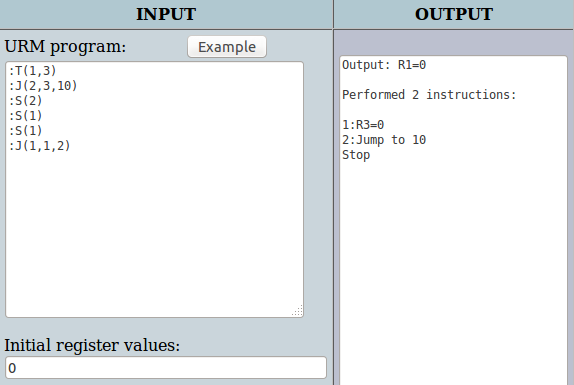
\includegraphics[scale=0.5]{images/80.png}
  	\end{figure}
	\subsection{Computación para la entrada $R1=1$}
	\begin{equation*}\begin{gathered}
	(1, <R1=1, R2=0, R3=0>) \sim (2, <R1=1, R2=0, R3=1>) \sim (3, <R1=1, R2=0, R3=1>) \sim\\
	(4, <R1=1, R2=1, R3=1>) \sim (5, <R1=2, R2=1, R3=1>) \sim (6, <R1=3, R2=1, R3=1>) \sim\\
	(2, <R1=3, R2=1, R3=1>) \sim (7, <R1=3, R2=1, R3=1>)
	\end{gathered}\end{equation*}
	\begin{figure}[H]
  		\centering
  		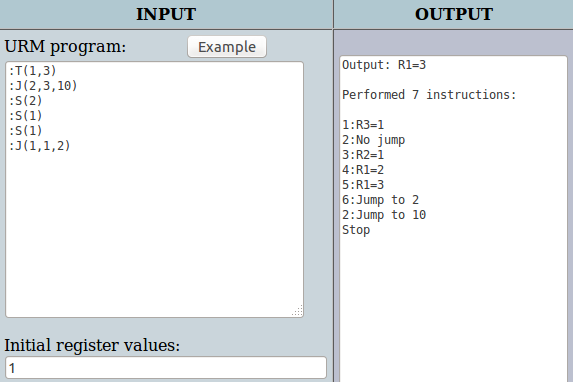
\includegraphics[scale=0.5]{images/81.png}
  	\end{figure}
	\subsection{Computación para la entrada $R1=2$}
	\begin{equation*}\begin{gathered}
	(1, <R1=2, R2=0, R3=0>) \sim (2, <R1=2, R2=0, R3=2>) \sim (3, <R1=2, R2=0, R3=2>) \sim\\
	(4, <R1=2, R2=1, R3=2>) \sim (5, <R1=3, R2=1, R3=2>) \sim (6, <R1=4, R2=1, R3=2>) \sim\\
	(2, <R1=4, R2=1, R3=2>) \sim (3, <R1=4, R2=1, R3=2>) \sim (4, <R1=4, R2=2, R3=2>) \sim\\
	(5, <R1=5, R2=2, R3=2>) \sim (6, <R1=6, R2=2, R3=2>) \sim (2, <R1=6, R2=2, R3=2>) \sim\\
	(7, <R1=6, R2=2, R3=2>)
	\end{gathered}\end{equation*}
	\begin{figure}[H]
  		\centering
  		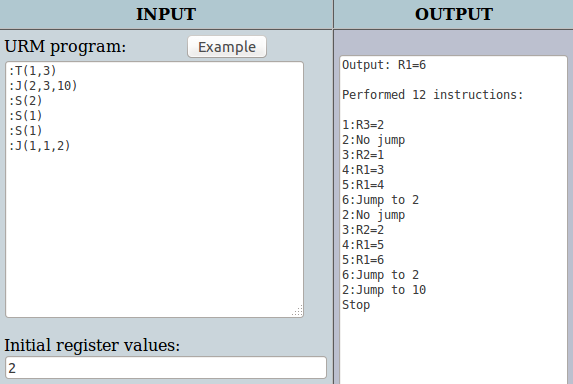
\includegraphics[scale=0.5]{images/82.png}
  	\end{figure}
	\subsection{Computación para la entrada $R1=3$}
	\begin{equation*}\begin{gathered}
	(1, <R1=3, R2=0, R3=0>) \sim (2, <R1=3, R2=0, R3=3>) \sim (3, <R1=3, R2=0, R3=3>) \sim\\
	(4, <R1=3, R2=1, R3=3>) \sim (5, <R1=4, R2=1, R3=3>) \sim (6, <R1=5, R2=1, R3=3>) \sim\\
	(2, <R1=5, R2=1, R3=3>) \sim (3, <R1=5, R2=1, R3=3>) \sim (4, <R1=5, R2=2, R3=3>) \sim\\
	(5, <R1=6, R2=2, R3=3>) \sim (6, <R1=7, R2=2, R3=3>) \sim (2, <R1=7, R2=2, R3=3>) \sim\\
	(3, <R1=7, R2=2, R3=3>) \sim (4, <R1=7, R2=3, R3=3>) \sim (5, <R1=8, R2=3, R3=3>) \sim\\
	(6, <R1=9, R2=3, R3=3>) \sim (2, <R1=9, R2=3, R3=3>) \sim (7, <R1=9, R2=3, R3=3>)
	\end{gathered}\end{equation*}
	\begin{figure}[H]
  		\centering
  		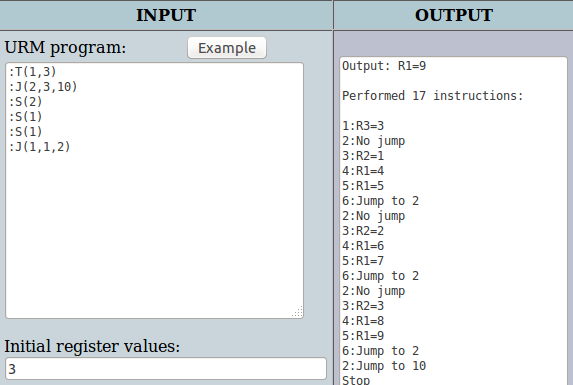
\includegraphics[scale=0.5]{images/83.png}
  	\end{figure}
	\subsection{Función calculada}
	El programa calcula la función
	\begin{equation*}
		f(x)=3x
	\end{equation*}
